\documentclass[tikz,border=8pt]{standalone}
\usepackage{amsmath}
\usepackage{amssymb}
\usetikzlibrary{arrows.meta,calc,decorations.pathreplacing,patterns,shapes.geometric,positioning,shadings,plotmarks}

\begin{document}
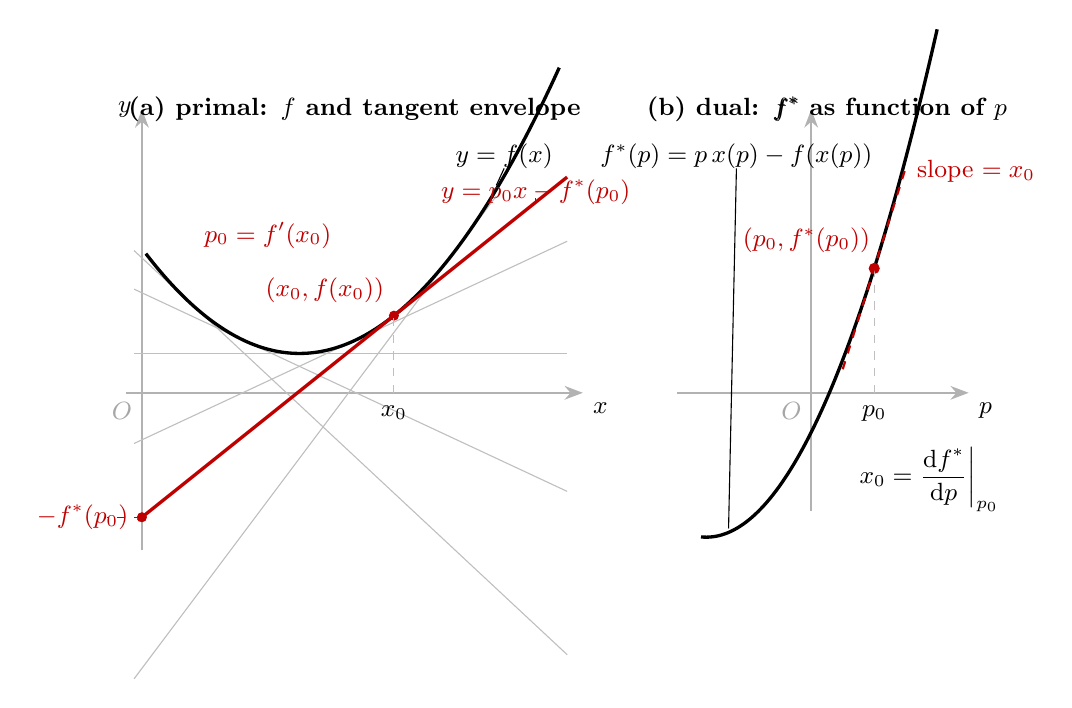
\begin{tikzpicture}[>=Stealth, font=\small]

% =================================================================
% LEFT PANEL: f(x) with tangent envelope
% =================================================================
\begin{scope}[xshift=0cm]

% f(x) = (x-2)^2/3 + 0.5 -- convex, smooth
% f'(x) = 2(x-2)/3
% At x0 = 3.2, p0 = 2*1.2/3 = 0.8
% f(3.2) = 1.44/3 + 0.5 = 0.98
% intercept b = f(x0) - p0*x0 = 0.98 - 0.8*3.2 = -1.58
% so -f*(p0) = -1.58, i.e. f*(p0) = 1.58

% axes
\draw[->, gray!60, thick] (-0.2,0) -- (5.6,0) node[below right, black] {$x$};
\draw[->, gray!60, thick] (0,-2.0) -- (0,3.6) node[left, black] {$y$};
\node[gray!70, below left] at (0,0) {$O$};

% gray tangent lines (envelope) at x = 0.6, 1.3, 2.0, 2.7, 4.0
% generic: tangent at xi: y = pi*x + (f(xi) - pi*xi)
% xi=0.6: pi=2*(-1.4)/3=-0.933, f=1.96/3+0.5=1.153, b=1.153-(-0.933*0.6)=1.713
% xi=1.3: pi=2*(-0.7)/3=-0.467, f=0.49/3+0.5=0.663, b=0.663-(-0.467*1.3)=1.270
% xi=2.0: pi=0, f=0.5, b=0.5
% xi=2.7: pi=2*0.7/3=0.467, f=0.49/3+0.5=0.663, b=0.663-0.467*2.7=-0.597
% xi=4.0: pi=2*2/3=1.333, f=4/3+0.5=1.833, b=1.833-1.333*4=-3.499

% gray tangents (drawn as straight lines clipped within frame)
\draw[gray!50, thin] (-0.1,{-0.933*(-0.1)+1.713}) -- (5.4,{-0.933*5.4+1.713});
\draw[gray!50, thin] (-0.1,{-0.467*(-0.1)+1.270}) -- (5.4,{-0.467*5.4+1.270});
\draw[gray!50, thin] (-0.1,{0*(-0.1)+0.5}) -- (5.4,{0*5.4+0.5});
\draw[gray!50, thin] (-0.1,{0.467*(-0.1)-0.597}) -- (5.4,{0.467*5.4-0.597});
\draw[gray!50, thin] (-0.1,{1.333*(-0.1)-3.499}) -- (4.5,{1.333*4.5-3.499});

% the curve f(x) = (x-2)^2/3 + 0.5
\draw[black, very thick, samples=80, domain=0.05:5.3, smooth, variable=\x]
   plot ({\x},{(\x-2)*(\x-2)/3 + 0.5});

% highlighted red tangent at x0 = 3.2, p0 = 0.8, b = -1.58
% line: y = 0.8 x - 1.58
\draw[red!75!black, very thick] (-0.05,{0.8*(-0.05)-1.58}) -- (5.4,{0.8*5.4-1.58});

% tangent point
\filldraw[red!75!black] (3.2,0.98) circle (1.6pt);
\node[red!75!black, above left=1pt and 0pt] at (3.2,0.98) {$(x_0,f(x_0))$};

% intercept marker on y-axis at -1.58
\filldraw[red!75!black] (0,-1.58) circle (1.6pt);
\draw[red!75!black, dashed, thin] (0,-1.58) -- (-0.45,-1.58);
\node[red!75!black, left] at (-0.05,-1.58) {$-f^{*}(p_0)$};

% x0 dashed projection
\draw[gray!50, dashed, thin] (3.2,0) -- (3.2,0.98);
\node[below] at (3.2,-0.04) {$x_0$};

% labels
\node[black] at (4.6,3.0) {$y=f(x)$};
\draw[black, thin] (4.6,2.85) -- (4.5,{(4.5-2)*(4.5-2)/3+0.5+0.05});

\node[red!75!black] at (5.0,2.55) {$y=p_0 x - f^{*}(p_0)$};
\draw[red!75!black, thin] (5.0,2.42) -- (5.0,{0.8*5.0-1.58+0.05});

\node[red!75!black] at (1.6,2.0) {$p_0=f'(x_0)$};

% panel title
\node[black] at (2.7,3.6) {\textbf{(a) primal: $f$ and tangent envelope}};

\end{scope}

% =================================================================
% RIGHT PANEL: f*(p) as function of p
% =================================================================
\begin{scope}[xshift=8.5cm]

% f*(p) is the Legendre dual of f(x)=(x-2)^2/3+0.5
% From f'(x) = 2(x-2)/3 = p, x(p) = 2 + 3p/2
% f*(p) = p*x(p) - f(x(p)) = p(2+3p/2) - [ (3p/2)^2/3 + 0.5 ]
%       = 2p + 3p^2/2 - 3p^2/4 - 0.5
%       = 2p + 3p^2/4 - 0.5
% domain we display p in [-1.4, 1.6]

% axes
\draw[->, gray!60, thick] (-1.7,0) -- (2.0,0) node[below right, black] {$p$};
\draw[->, gray!60, thick] (0,-1.5) -- (0,3.6) node[left, black] {$f^{*}$};
\node[gray!70, below left] at (0,0) {$O$};

% the dual curve
\draw[black, very thick, samples=80, domain=-1.4:1.6, smooth, variable=\p]
   plot ({\p},{2*\p + 0.75*\p*\p - 0.5});

% point at p0 = 0.8, f*(p0) = 1.6 + 0.48 - 0.5 = 1.58
\filldraw[red!75!black] (0.8,1.58) circle (1.8pt);
\node[red!75!black, above left=2pt and -2pt] at (0.8,1.58) {$(p_0,f^{*}(p_0))$};

% mark p0 on the axis
\draw[gray!50, dashed, thin] (0.8,0) -- (0.8,1.58);
\node[below] at (0.8,-0.04) {$p_0$};

% slope of f* at p0 is x0 = 3.2 (duality)
% draw a small slope-indicator at the red point: tangent line of f* at p0
% slope = df*/dp = 2 + 3p/2 = 2 + 1.2 = 3.2 = x_0
\draw[red!75!black, dashed, thick] (0.4,{1.58-3.2*0.4}) -- (1.2,{1.58+3.2*0.4});
\node[red!75!black, right] at (1.22,{1.58+3.2*0.4-0.05}) {slope $= x_0$};

% label for the curve
\node[black] at (-0.95,3.0) {$f^{*}(p)=p\,x(p)-f(x(p))$};
\draw[black, thin] (-0.95,2.85) -- (-1.05,{2*(-1.05)+0.75*(-1.05)*(-1.05)-0.5+0.05});

\node[black] at (1.5,-1.1) {$x_0=\dfrac{\mathrm{d}f^{*}}{\mathrm{d}p}\bigg|_{p_0}$};

% panel title
\node[black] at (0.2,3.6) {\textbf{(b) dual: $f^{*}$ as function of $p$}};

\end{scope}

\end{tikzpicture}
\end{document}
